\chapter{Návrh herního systému}
\label{chap:design}

Na základě požadavků stanovených v předchozí kapitole byl vytvořen návrh herního systému, který je pro přehlednost rozdělen do několika částí. První část se zabývá komponenty hry, druhá část se zaměřuje na herní mechaniky a třetí část se věnuje propojení s webovou aplikací.

Hybridní deskové hře, která je finálním produktem této práce, bylo určeno pracovní jméno \textit{Trails Through Shadows} (zkratkou \textit{TTS}). Dále je však zmiňována především pod názvem \textit{modelová hra}.


\section{Schéma hry}
\label{sec:design_scheme}

Na návrhu databáze pracoval celý tým vyvíjející modelovou hru, jeho rozvržení je však skvělým nástrojem pro popsání návrhu herních modelů, proto bude detailně rozebráno v následující sekci.

\begin{figure}[h]
    \centering
    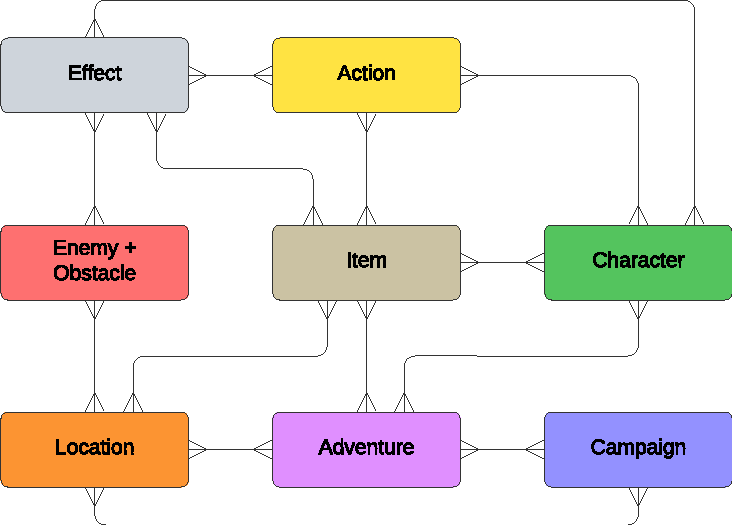
\includegraphics[scale=0.8]{../../shared/diagrams/er_macro.pdf}
    \caption{Makro pohled na schéma databáze}
    \label{diag:er_macro}
\end{figure}

Na schématu \ref{diag:er_macro} je orientačně zobrazen makro pohled na schéma databáze, které je pro přehlednost rozděleno do několika barevně rozlišených částí, neboť celková databáze zahrnuje 45 tabulek. Každá z těchto částí je následně podrobněji popsána v následujících podsekcích.


\subsection{Akce}
\label{subsec:schema_actions}

Popis celkového rozvržení herních komponent začíná schématem \ref{diag:er_action}, které definuje strukturu \textbf{akcí}, jejichž mechanická funkcionalita je dále rozepsána v sekci \ref{subsec:design_actions}. Každá akce má svůj název \attr{title} a popis \attr{description}, který hráči pomůže pochopit, co daná akce přibližně znamená, bez nutnosti hlubšího studia samotné karty. Dále je v akci uchována informace o jejím zahození \attr{discard}, která určuje, v jakém případě a na jak dlouho musí hráč po odehrání danou kartu zahodit. Každá akce má také požadovanou úroveň \attr{levelReq}, která umožňuje tvorbu akcí, které hráči mohou odemykat spolu s postupem příběhem.

\begin{figure}[h]
    \centering
    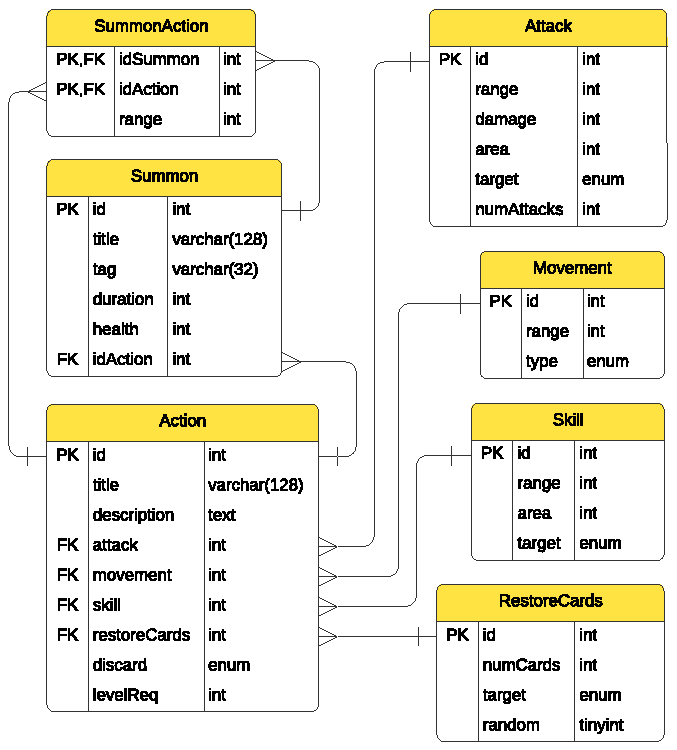
\includegraphics[scale=0.8]{../../shared/diagrams/er_action.pdf}
    \caption{Schéma akcí}
    \label{diag:er_action}
\end{figure}

V modelové hře se akce skládají z pěti částí, interně nazývanými \textit{features} neboli \textit{prvky akce}. Jedná se o \textit{pohyb}, \textit{útok}, \textit{schopnost}, \textit{summon} a \textit{obnovení karet}. Každý z prvků je nepovinný a může být v akci využit maximálně jednou s výjimkou summonů, kterých může jedna akce vyvolat libovolný počet. Samotní summoni poté také mají svou vlastní akci, kterou ve svém kole konají. Průběh jednotlivých prvků je popsán v sekci \ref{subsec:design_actions}.


\subsection{Postavy}
\label{subsec:schema_character}

Na diagramu \ref{diag:er_character} je zobrazeno schéma nejen postav, ale i předmětů, neboť jsou k sobě úzce vázány. 

\begin{figure}[h]
    \centering
    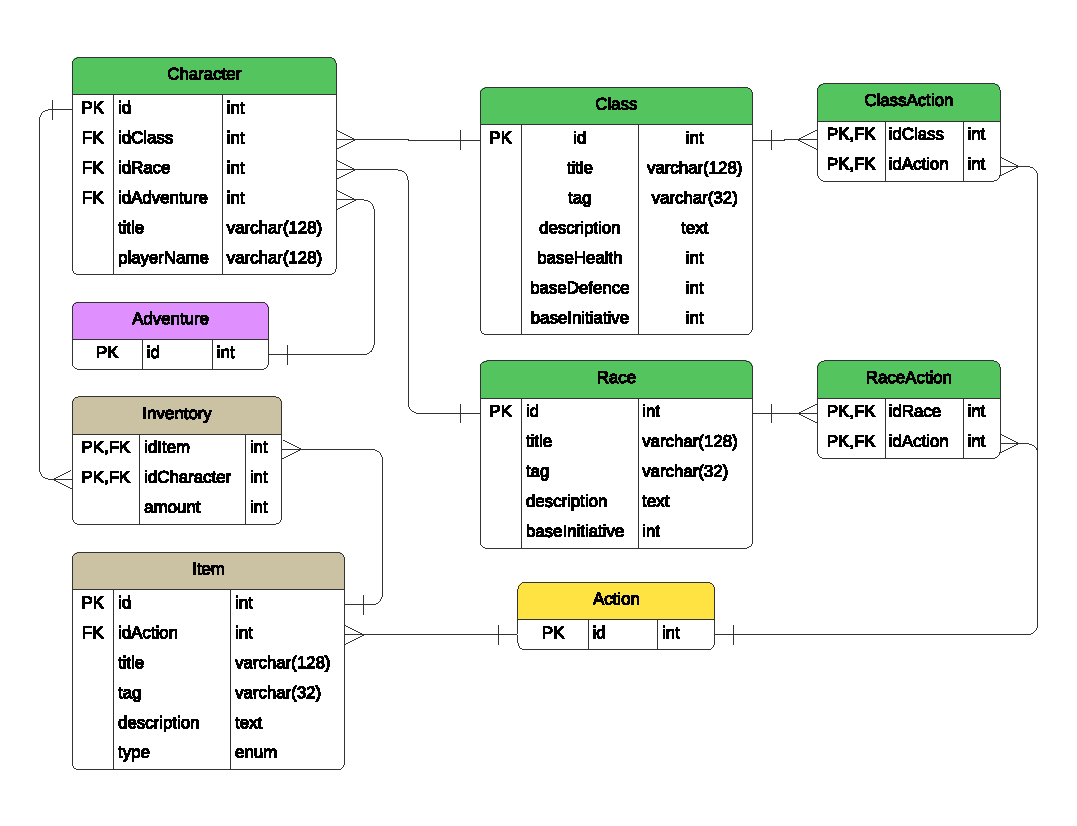
\includegraphics[scale=0.8]{../../shared/diagrams/er_character.pdf}
    \caption{Schéma postav}
    \label{diag:er_character}
\end{figure}

\textbf{Postava} má několik základních vlastností, které ji definují -- jméno postavy \attr{title} a jméno hráče \attr{playerName}, dále je však každá postava složena z kombinace \textbf{rasy} a \textbf{třídy}. Obě tyto tabulky obsahují jméno \attr{title}, popis \attr{description} a štítek \attr{tag}, který slouží k identifikaci obrázku, který jim přísluší. U obou je také zaznamenána základní iniciativa, třída však obsahuje také definici základního zdraví a obrany postavy. Postava je vždy vázána na jedno určité dobrodružství.

Každá postava může mít také vybavení, které je k ní navázáno přes \textbf{inventář}, kde se zaznamenává, kolik kterého typu předmětu postava má. Samotné \textbf{předměty} jsou podobně jako rasy a třídy složeny z názvu, popisu a štítku, kromě toho však také obsahují informaci o jejich typu \attr{type}, který určuje, zda se jedná o zbraň, brnění nebo jiný typ předmětu.

Předměty, rasy a třídy mohou být chápány jako možnosti získání určitých akcí, neboť všechny tři tabulky mají na akce vazbu. Rasa a třída může hráči poskytovat neomezené množství akcí, předmět však má vždy jen jednu akci, kterou hráč může využít, což je limitace zavedená z důvodu přehlednosti fyzických komponent, popsaných v sekci \textbf{//TODO}.


\subsection{Lokace}
\label{subsec:schema_location}

Schéma lokací je zobrazeno na diagramu \ref{diag:er_location}, které je díky velkému množství složených primárních klíčů složené z mnoha vazeb, i přes jejich četnost však není nijak zvlášť komplikovaný.

\begin{figure}[h]
    \centering
    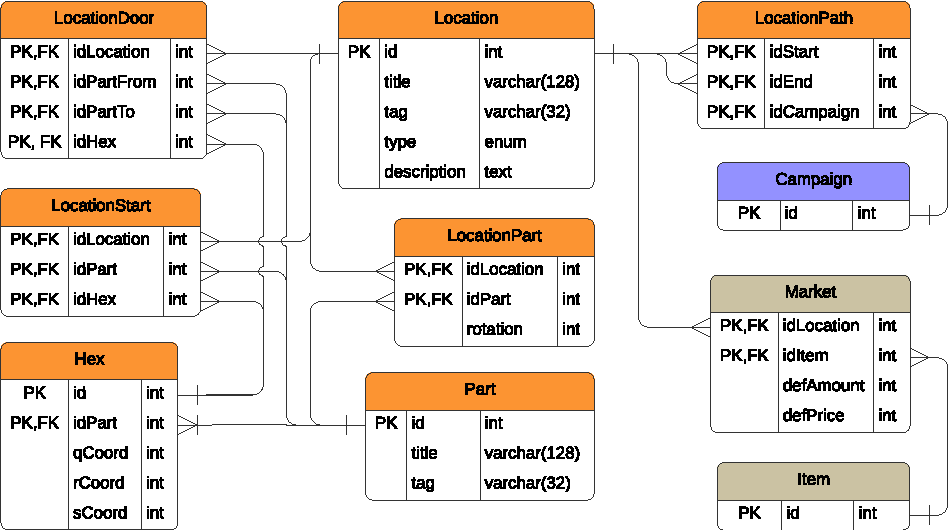
\includegraphics[scale=0.8]{../../shared/diagrams/er_location.pdf}
    \caption{Schéma lokací}
    \label{diag:er_location}
\end{figure}

\textbf{Lokace} je základním prvkem hry, který hráči umožňuje prozkoumávat herní svět. Ve své podstatě se jedná o místo na herní mapě, které se hráči mohou navštívit. Každá lokace má své jméno \attr{title}, popis \attr{description} a štítek \attr{tag}, podobně jako předchozí entity. Dále si nese informaci o typu \attr{type}, jenž určuje, zda se jedná o lokaci se soubojem \attr{encounter} nebo o obchod \attr{market}, nejčastěji se však používá první možnost, pro kterou se poté využívají ostatní tabulky pro zápis herní plochy.

Každá lokace se skládá z několika \textbf{částí} mapy \attr{Part}, které mohou být na stole různě otočené, proto je jejich rotace \attr{rotation} také zaznamenaná. Části mají opět nejen jméno ale i štítek, který má tentokrát ještě další funkcionalitu, neboť představuje identifikátor, který umožňuje hráčům snadno najít odpovídající části mapy mezi ostatními herními komponentami. Herní pole je dále rozděleno na \textbf{hexagony}, u kterých bylo rozhodnuto o použití tzv. kubického souřadného systému, který polím ve 2D prostoru přiřadí 3D souřadnice (\texttt{q}, \texttt{r}, \texttt{s}), což usnadňuje výpočty pro herní mechaniky, které se týkají pohybu a vzdáleností mezi jednotlivými políčky.

Jak jde vidět z diagramu, lokace jsou spolu s ostatními tabulkami vázány spoustou vazeb, které umožňují hlubší specifikaci propojení. Jedná se například o reprezentaci dveří spojující části herní desky v rámci lokace \attr{LocationDoor}, počáteční políčka lokace, kde se na začátku souboje umisťují postavy hráčů \attr{LocationStart}, nebo propojení s kampaní, v rámci které jsou na sebe lokace dynamicky navázány ve světové mapě \attr{LocationPath}. Speciálním případem vazební tabulky je pak obchod \attr{Market}, který pro danou lokaci určuje nabízené předměty, jejich množství a ceny.

\subsubsection*{Nepřátelé a překážky}
\label{subsubsec:schema_enemy_obstacle}

Lokace jsou zaplněny nepřáteli \attr{Enemy} a překážkami \attr{Obstacle}, jak je možné vyčíst z diagramu \ref{diag:er_enemy_obstacle}. Obě dvě entity opět obsahují informace o názvu, popisu a štítku pro vyhledávání obrázků a také mají vazbu na hexagon neboli políčko určité lokace, na které se vyskytují (\texttt{HexEnemy} a \texttt{HexObstacle}), dále se však mírně liší.

\begin{figure}[h]
    \centering
    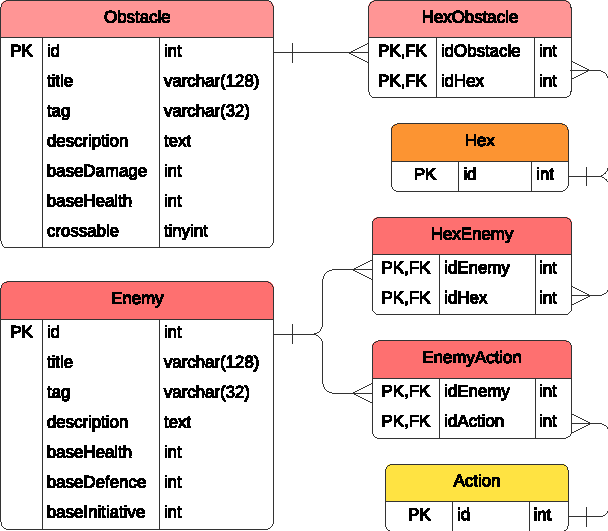
\includegraphics[scale=0.8]{../../shared/diagrams/er_enemy_obstacle.pdf}
    \caption{Schéma nepřátel a překážek}
    \label{diag:er_enemy_obstacle}
\end{figure}

\textbf{Nepřátelé} v podstatě kopírují statistiky postav, mají své vlastní zdraví, obranu a iniciativu. Dále také mohou mít své vlastní akce, které budou v souboji provádět \attr{EnemyAction}.

\textbf{Překážky} jsou oproti nim pasivní, proto mají zaznamenané pouze své zdraví a míru zranění, které dostane entita, která se na ní zraní. Také má indikátor toho, zda je tato překážka průchozí \attr{crossable} nebo nikoliv.


\subsection{Kampaň}
\label{subsec:schema_campaign}

Kampaň slouží k reprezentaci celého příběhu, kterým si hráči budou v rámci modelové hry procházet. Její schéma je vyobrazeno na diagramu \ref{diag:er_campaign}.

\begin{figure}[h]
    \centering
    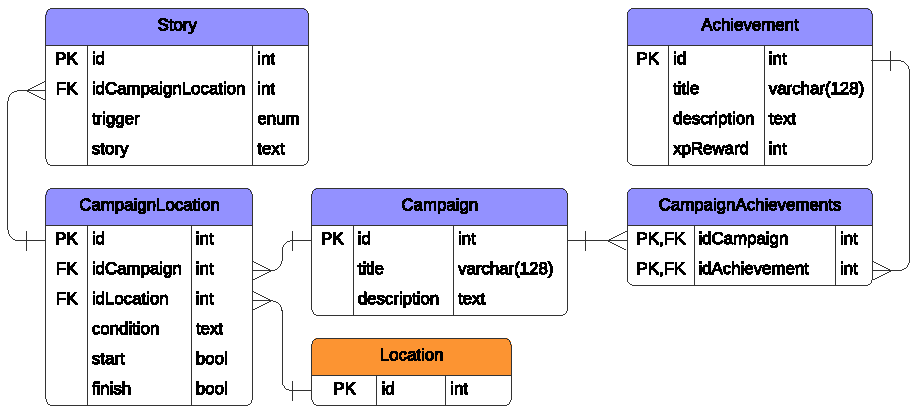
\includegraphics[scale=0.8]{../../shared/diagrams/er_campaign.pdf}
    \caption{Schéma kampaně}
    \label{diag:er_campaign}
\end{figure}

Samotná \textbf{kampaň} si moc dat nenese, obsahuje pouze název a popis. Klíčová je však především její vazba na lokace \attr{CampaignLocation}, které jsou v rámci kampaně propojeny do světové mapy. Tato vazební tabulka obsahuje informace o tom, jaké lokace jsou v rámci kampaně dostupné, zda se jedná o počáteční \attr{start} nebo případně konečnou \attr{finish} lokaci daného příběhu a také jaké jsou podmínky pro dokončení či selhání lokace \attr{condition}. K této vazbě se také připojuje příběh \attr{Story}, který se může spouštět po určitých událostech odehraných v rámci lokace.

Za zmínku také stojí herní \textbf{úspěchy} \attr{Achievement}, které jsou taktéž navázány na kampaň. Jedná se o určité cíle, které hráči mohou splnit v rámci hry a za jejichž dokončení získají odměnu. Tento cíl si vždy nese název, krátký popis a také odměnu v podobě zkušeností.


\subsubsection*{Dobrodružství}
\label{subsubsec:schema_adventure}

Rozehranou kampaň, ve které již hráči dělají příběhový postup, reprezentuje tzv. \textbf{dobrodružství} \attr{Adventure}, které je zobrazeno na diagramu \ref{diag:er_adventure}.

\begin{figure}[h]
    \centering
    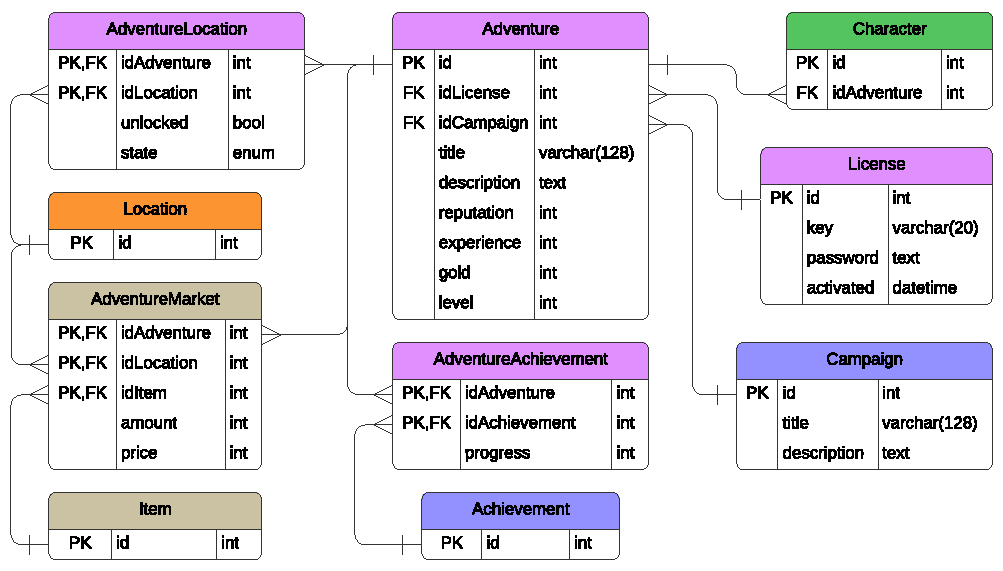
\includegraphics[scale=0.8]{../../shared/diagrams/er_adventure.pdf}
    \caption{Schéma dobrodružství}
    \label{diag:er_adventure}
\end{figure}

Samotná tabulka dobrodružství je relativně objemná, obsahuje kromě klasického názvu a popisu také statistiky rozehrané kampaně, jako je reputace \attr{reputation}, zkušenosti \attr{experience}, peníze \attr{gold} a také úroveň družiny \attr{level}. Úspěchy určité kampaně \attr{AdventureAchievement} se zde taktéž uchovávají spolu s číslem určující postup v daném cíli \attr{progress}.

Vazba na lokace \attr{AdventureLocation} v sobě drží informace o tom, které již byly odemčeny \attr{unlocked} a v jakém stavu \attr{state} jsou, ať už dokončené nebo zatím neúspěšné. Pro podporu dynamičnosti herního rozvoje je zde také možnost upravovat zásoby a ceny obchodů \attr{AdventureMarket}, které jsou dále vázány na samotné předměty.

Jak již bylo řečeno výše, dobrodružství se může účastnit několik postav. Kromě toho má však dobrodružství nastavenou i \textbf{licenci} \attr{License}, se kterou ho je možné spustit \attr{AdventureLicense}. Licenční klíče jsou náhodně generovaná sekvence dvaceti znaků, které budou distribuovány spolu se hrou a umožní hráčům změnit si heslo, pomocí kterého se budou do systému přihlašovat. Takto bude zajištěno, že hráči mají přístup pouze na své postavy a příběhy a zároveň se znemožní nelegální kopírování hry.


\subsection{Efekty}
\label{subsec:schema_effect}

Posledním prvkem, který je nutné zmínit, jsou \textbf{efekty} \attr{Effect}, popsány na diagramu \ref{diag:er_effect}.

\begin{figure}[h]
    \centering
    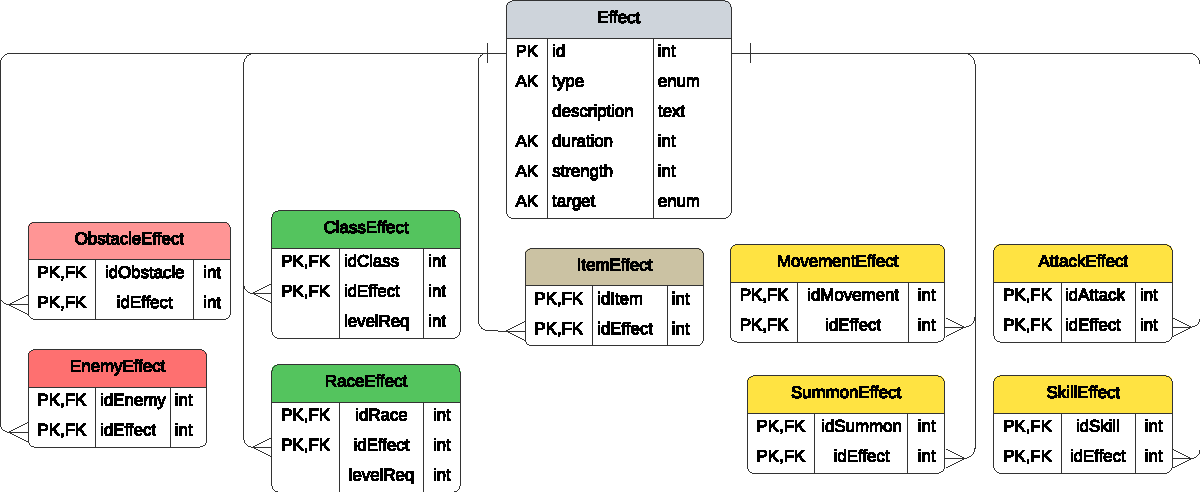
\includegraphics[scale=0.76]{../../shared/diagrams/er_effect.pdf}
    \caption{Schéma efektů}
    \label{diag:er_effect}
\end{figure}

Efekty prolínají celou strukturu hry, proto nebyly zapsány do jednotlivých grafů výše, ale všechny jejich vazby byly zahrnuty v tomto diagramu. 

Hlavní charakteristikou efektu je typ \attr{type}, jejichž mechanická implementace je popsána v sekci \ref{subsec:design_effects}. Je zde také možnost hráčům předložit popis efektu \attr{description}, který jim pomůže pochopit, co daný efekt znamená. Dále se zaznamenává síla a trvání efektu a také cíl, na který efekt míří.

Efekty mohou být aplikovány na překážky, nepřátele, třídy a rasy, předměty a většinu prvků akce -- pohyb, útok, schopnost a summon. U rasy a třídy je navíc přidán atribut minimální úrovně \attr{levelReq}, který umožňuje postavám odemykat nové pasivní efekty s rostoucí úrovní.


\section{Herní mechaniky}
\label{sec:design_mechanics}

Mechaniky modelové hry jsou silně inspirované především výše zmíněnou deskovou hrou \glsref{gloomhaven}, ale jsou upravené tak, aby lépe vyhovovaly stanoveným požadavkům.


\subsection{Souboj}
\label{subsec:design_encounter}

Souboj je hlavní funkcionalitou, kterou hra nabízí. Průběh souboje je rozdělen do několika fází, které jsou znázorněny na diagramu \ref{diag:encounter}. Ještě před samotným hraním si systém zaznačí, že lokace už byla navštívena (\texttt{visited}), pokud již nemá nastavený jiný stav, který je důležitější (jako například \texttt{completed} nebo \texttt{failed}). Následně hráčům zobrazí příběh, který je s touto lokací spojený.

Poté následuje fáze přípravy hrací desky. Systém zobrazí počáteční místnost lokace, všechny nepřátele, překážky a dveře, které se v ní vyskytují spolu s identifikátory, které umožní hráčům tyto části jednoduše najít a sestavit tak odpovídající konfiguraci místnosti na herním stole. Když je všechno připraveno, hráči umístí své postavy na políčka určená pro hráče a s tím je příprava herního pole hotová.

\newpage
\begin{figure}[H]
    \centering
    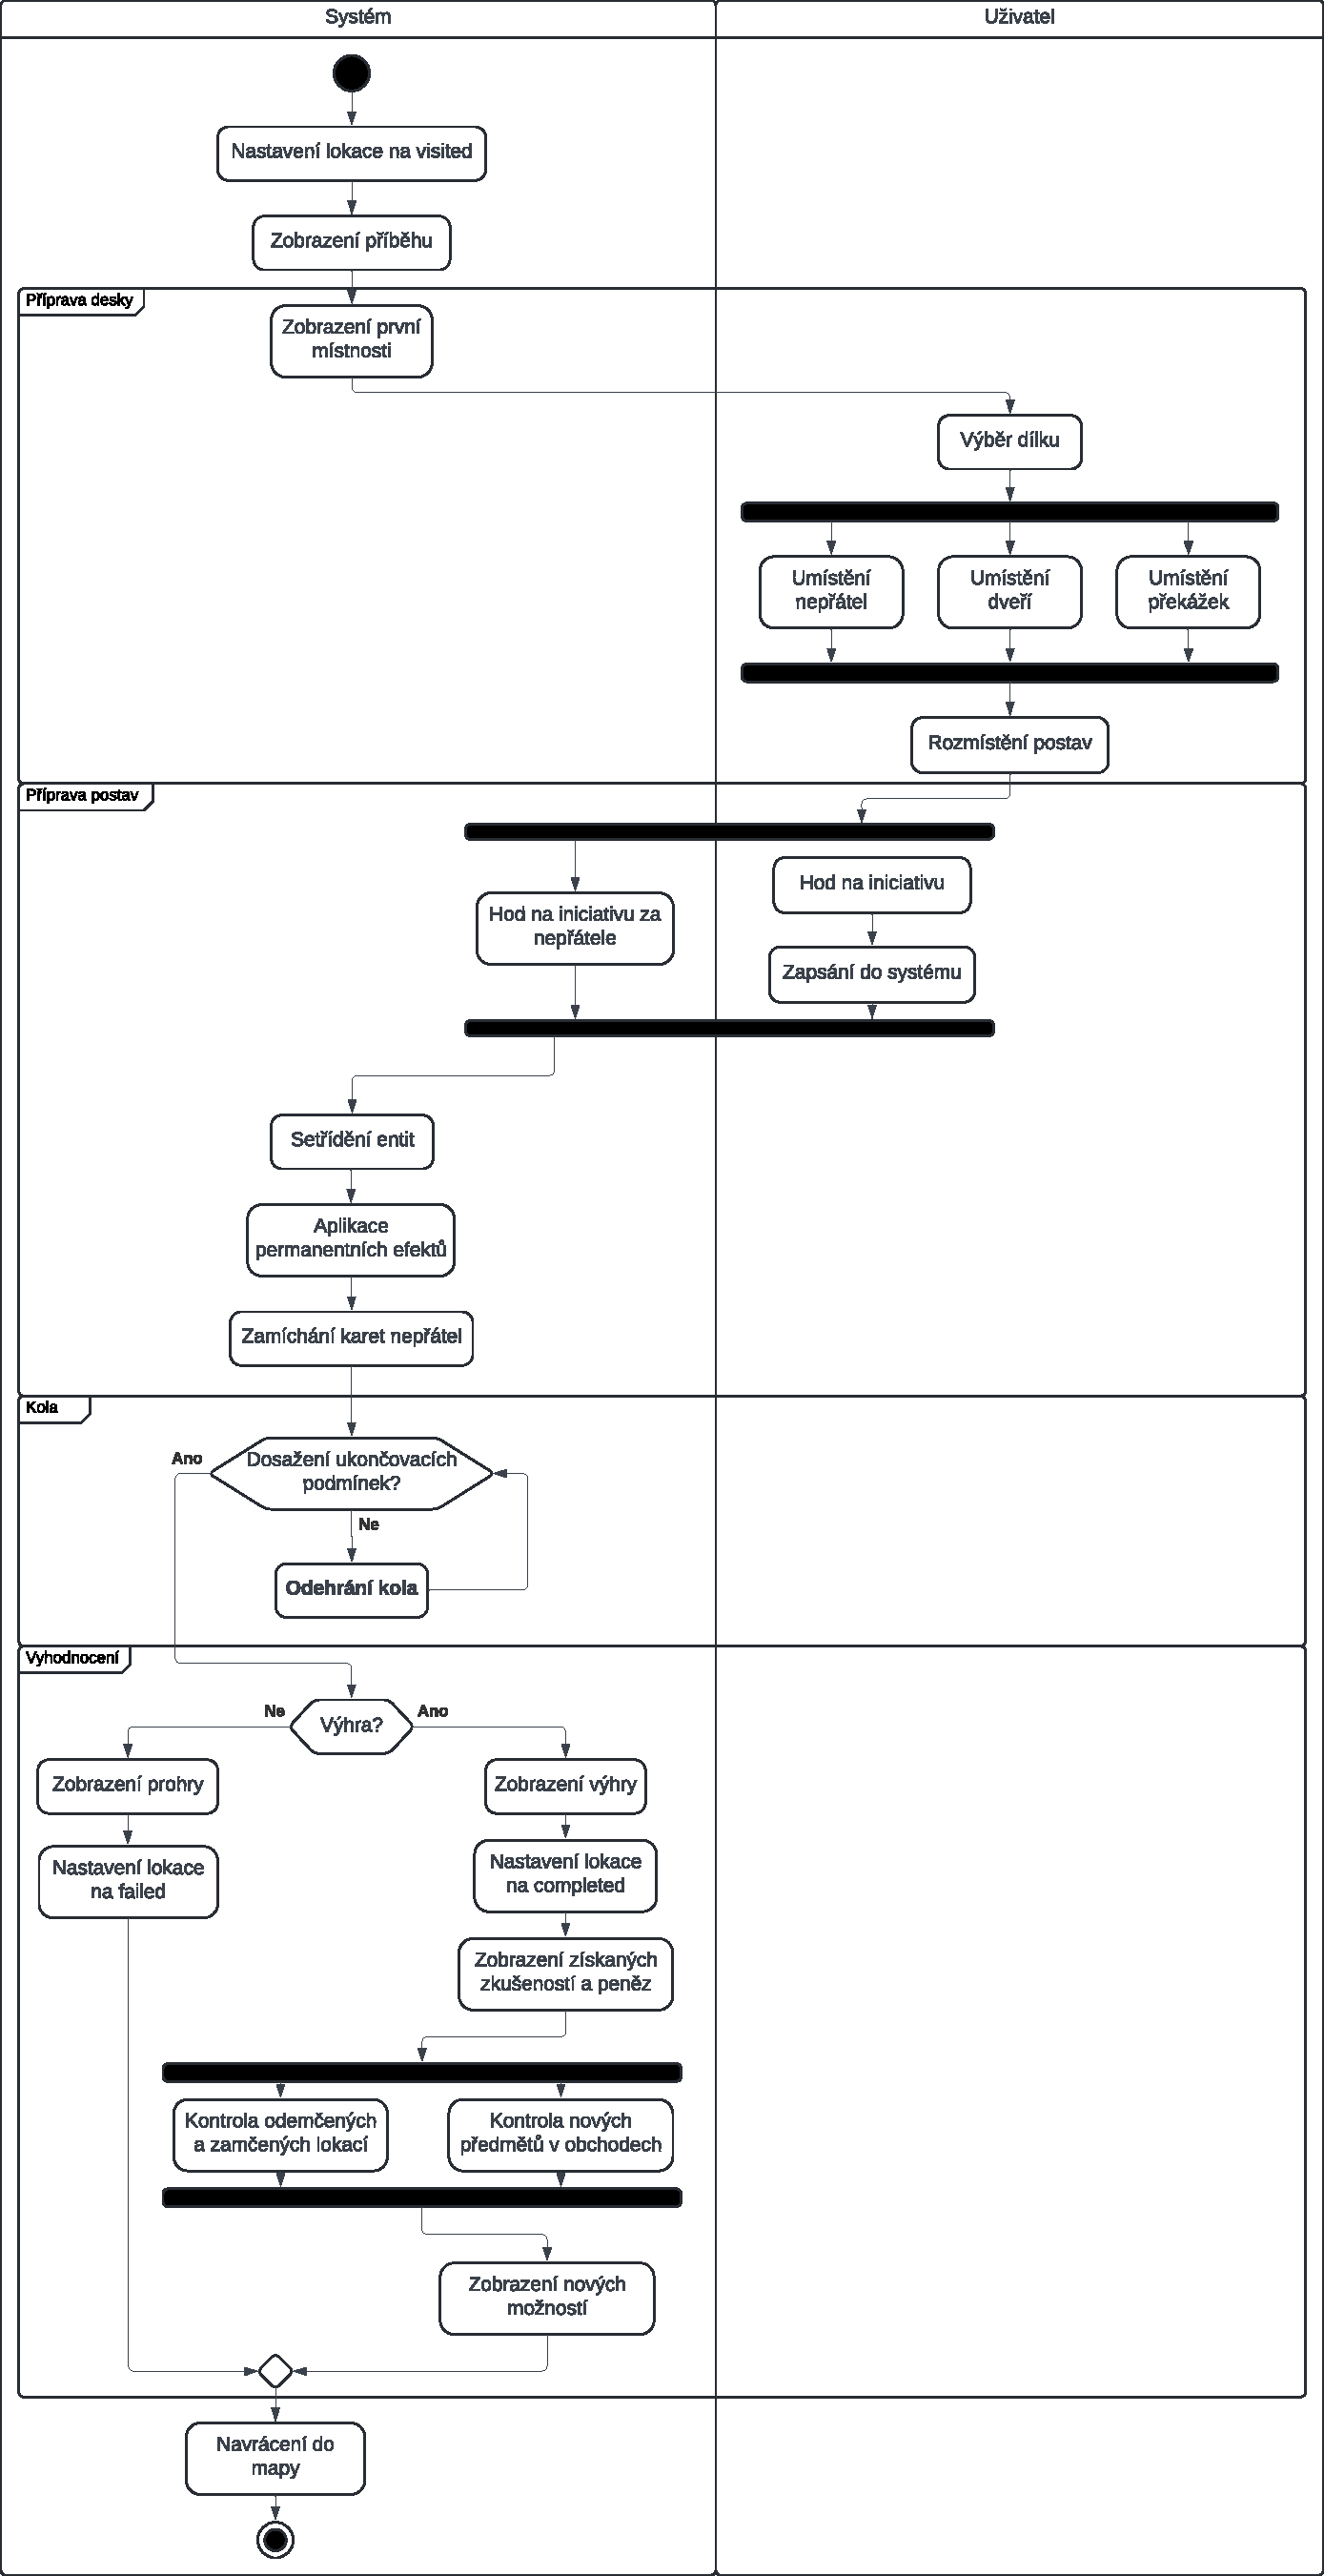
\includegraphics[height=0.98\textheight]{figures/diagrams/encounter.pdf}
    \caption{Diagram průchodu lokací}
    \label{diag:encounter}
\end{figure}
\newpage

Druhá část přípravy je věnována samotným postavám a nepřátelům a tvorbě iniciativního žebříčku. Každý s hráčů si hodí svou kostkou na iniciativu a zaznamená výsledek do systému, který tento modifikátor automaticky přičte k základní výši iniciativy, který hráčova postava získala ze své rasy, třídy a vybavení. Za nepřátele toto provede systém automaticky. Výsledný žebříček je seřazen sestupně a hráči a nepřátelé se podle něj střídají v rámci kola. Dále se tu také provádí aplikace permanentních efektů, tedy efektů získaných ze zázemí a předmětů u postav nebo vrozené efekty u nepřátel, podle diagramu \ref{diag:apply_effect}. Systém pak ještě zamíchá simulovaný balíček nepřátelských karet, který bude sloužit k určení jejich akcí.

Následuje fáze kol, která se provádí podle diagramu \ref{diag:round} opakovaně ve smyčce, dokud hráči nesplní jistou předem určenou ukončovací podmínku.

Po dosažení této podmínky systém vyhodnotí, jak hra skončila. Pokud se jedná o prohru, zobrazí tuto informaci hráčům a nastaví stav lokace na \texttt{failed}. Pokud ovšem hráči lokaci zdolali úspěšně, systém provede kontrolu nových lokací a předmětů v obchodech, které hráči dokončením tohoto souboje odemkli nebo naopak zablokovali. Pomocí tohoto mechanismu se zajišťuje, že hra bude mít dynamický průběh a hráči budou mít motivaci prozkoumávat nové lokace a plnit úkoly. Po této kontrole systém hráčům zahlásí co vše jejich úspěch změnil, jaké mají nové možnosti a kolik peněz a zkušeností svou výhrou získali. Na závěr systém přehraje příběh konce této lokace a navrátí hráče zpět do mapy, kde mohou pokračovat v průzkumu světa.


\subsection{Kola}
\label{subsec:design_rounds}

\begin{figure}[H]
    \centering
    \includeplantuml[scale=0.7]{round}
    \caption{Diagram kola}
    \label{diag:round}
\end{figure}

V rámci herního kola se nejprve provádí tahy hráčů a nepřátel v pořadí iniciativy podle diagramů \ref{diag:player_turn} a \ref{diag:enemy_turn}. Když tahy dojdou na konec iniciativy, systém zkontroluje, zda některý z hráčů během svého kola neotevřel dveře. Pokud ano, pak je hráčům zobrazena nově odhalená místnost, jejíž desku, nepřátele, překážky a dveře si opět podle identifikátorů rozloží na herní stůl, čímž se herní plocha rozšíří. Systém následně přidá nové nepřátele do iniciativního žebříčku a zamíchá jejich karty. Pokud hráči dveře neotevřeli, systém přeskočí tuto fázi, po které již kolo končí.


\subsection{Tahy}
\label{subsec:design_turns}

\begin{figure}[H]
    \centering
    \includeplantuml[scale=0.7]{playerTurn}
    \caption{Diagram herního tahu hráče}
    \label{diag:player_turn}
\end{figure}

Tah hráče je vyobrazen na diagramu \ref{diag:player_turn}. Během začátku a konce se systém věnuje efektům, jejichž vyhodnocení a uvolnění je popsáno v kapitole \ref{subsec:design_effects}, a také summonům, což uvolňuje čas, který by jinak musel být stráven jejich monitorováním. Samotný hráč má nejprve za úkol vybrat si dvě karty, které v tomto kole bude chtít zahrát. Následně akce na kartách vyhodnotí podle diagramů popsaných v kapitole \ref{subsec:design_actions} a pokud má na stole vyložené nějaké karty vyvolaných summonů, zahraje také jejich akce. Veškeré akce může vykonat v libovolném pořadí, což mu dává možnost plánovat své tahy tak, aby byly co nejefektivnější. Pokud během vykonávání akcí dojde k změně stavu jakékoliv entity na herní desce, hráč tyto změny zaznamená a pokračuje v dalších akcích. Po vykonání všech akcí hráč zahodí zahrnuté karty podle jejich zahazovacího pravidla, čímž své kolo ukončí.

\begin{figure}[H]
    \centering
    \includeplantuml[scale=0.7]{enemyTurn}
    \caption{Diagram herního tahu nepřítele}
    \label{diag:enemy_turn}
\end{figure}

Tah nepřítele znázorněn na diagramu \ref{diag:enemy_turn} je oproti tomu hráčskému mnohem jednodušší. Nepřátelé mají svůj vlastní balík karet, ze kterého jim systém vybere jednu, kterou v daném kole zahrají. Jedná se o simulaci reálného karetního balíčku, takže pokud v něm karty dojdou, opět se všechny zamíchají a tahají se znova. Na hráčích pak závisí, aby vyhodnotili, jakým způsobem se nepřátelé pohnou a na koho zaútočí, ale musí se řídit instrukcemi, které od systému dostali. Jakékoli změny musí být opět propsány do systému, který se zde také stará o vyhodnocení efektů.


\subsection{Akce}
\label{subsec:design_actions}

Jak již bylo znázorněno na schématu \ref{diag:er_action}, akce jsou strukturovány do pěti prvků, které mohou ale také nemusí být v akci využity. Vyhodnocení akce spočívá v provedení všech těchto prvků dle uvážení hráče, přičemž si může vybrat nejen to, jak se k jednotlivým prvkům jeho postava zachová, ale také v jakém pořadí je provede.

\begin{figure}[H]
    \centering
    \includeplantuml[scale=0.7]{movement}
    \caption{Diagram pohybu}
    \label{diag:movement}
\end{figure}

Na prvním diagramu \ref{diag:movement} je zobrazen průběh \textbf{pohybu}. Před samotným vyhodnocením systém hráči předá informaci o bonusové rychlosti nebo případně zpomalení jeho postavy, což je možné získat z aktivních efektů nebo vybavení postavy. Hráč tento bonus přičte k číslu, které má napsané na kartě pohybu a posune se po herním poli o odpovídající počet polí. Pohyb má tři typy -- \textit{chůze}, \textit{skok} a \textit{teleportace}. Chůze je základním typem pohybu, skok je pohyb, který umožňuje přeskočit překážku nebo nepřítele a teleportace je pohyb, který umožňuje postavě přesunout se na libovolné místo na herním poli i přes zdi, ale samozřejmě pořád v limitu polí. Pokud postava po své cestě přejde přes překážku, musí na sebe vzít její efekt a tuto skutečnost zaznamenat do systému.

\begin{figure}[H]
    \centering
    \includeplantuml[scale=0.7]{attack}
    \caption{Diagram útoku}
    \label{diag:attack}
\end{figure}

Průběh \textbf{útoku} znázorňuje diagram \ref{diag:attack}. Před útokem systém opět zjistí, zda má postava nějaký bonus k útoku, který může získat z aktivních efektů nebo vybavení, a v takovém případě tento bonus hráči zobrazí. Hráč si poté vybere cíl a může na něj zaútočit tolikrát, kolik určuje jeho karta útoku. Při každém zaútočení se cíli aplikuje nejen velikost zranění, ale také všechny efekty, které útok může způsobovat. Tyto efekty však nejsou hlavní součástí útoku, proto ve většině případů nejsou na této kartě zaznamenány. Veškeré zranění nebo získané efekty, které cíl utrpí, musí být zaznamenány do systému.

\begin{figure}[H]
    \centering
    \includeplantuml[scale=0.7]{skill}
    \caption{Diagram schopnosti}
    \label{diag:skill}
\end{figure}

Zjednodušenou verzí útoku je \textbf{schopnost}, která je znázorněna na diagramu \ref{diag:skill}. Oproti útoku je plně zaměřena pouze na efekty, musí tedy mít alespoň jeden, může se jednat například o zapálení cíle, ale také o vyléčení postavy. Po jejím zahrání musí hráč zaznamenat všechny efekty, které schopnost způsobila.

\begin{figure}[H]
    \centering
    \includeplantuml[scale=0.7]{summon}
    \caption{Diagram summona}
    \label{diag:summon}
\end{figure}

\textbf{Vyvolání summona}, znázorněno na diagramu \ref{diag:summon}, je jednou z komplexnějších prvků akce, které mají hráči k dispozici, ale pořád je intuitivně pochopitelná. Uživatel opět začne vybráním cíle, tentokrát se však jedná o políčko v dosahu uvedeném na kartě, na které bude svého poskoka vyvolávat. Poté najde odpovídající figurku, umístí ji na vybrané pole a kartu, pomocí které summona vyvolal, položí na stůl před sebe. Když pak dojde na jeho tah, může pomocí této karty provést odpovídající akci i za svého summona. Na závěr nově vyvolanou entitu zaznamená do systému, který si ho uloží a zobrazí jej v žebříčku iniciativy pod jménem hráče, který ho vyvolal. Po vyvolání má hráč možnost ihned zahrát tah summona, což mu umožňuje získat výhodu v boji.

\begin{figure}[H]
    \centering
    \includeplantuml[scale=0.7]{restoreCards}
    \caption{Diagram obnovení karet}
    \label{diag:restore_cards}
\end{figure}

Posledním prvkem akce, který hráči mohou využít, je \textbf{obnovení karet}, pomocí něhož si mohou do ruky vrátit karty, které v předchozích tazích zahodili. Jak je možné vidět na diagramu \ref{diag:restore_cards}, celý postup zde provádí pouze hráč bez asistence systému. Nejprve si vybere cíl obnovení, což může být jeho postava nebo postava jiného hráče, a poté vybere karty, které chce vrátit. Na kartě je určen počet karet, které může hráč obnovit, a také příznak náhody, podle které se vybírají karty buď náhodně, nebo si cíl může sám vybrat, které karty chce získat zpět. Tímto způsobem vybrané karty si cíl poté vrátí do ruky a může je využít v dalších tazích.



\subsection{Efekty}
\label{subsec:design_effects}

Modelová hra obsahuje několik druhů efektů, které mohou entity na herním poli ovlivnit. Tyto efekty mohou být aplikovány na postavy, nepřátele nebo summony a mohou mít různé účinky. Jejich výčet je uveden v tabulce \ref{tab:effects}.

Každý efekt má dvě základní vlastnosti, které ho popisují. První z nich je \textit{Strength}, která určuje, jak silný je efekt, což je využito s rozličnými účely u různých typů efektu. Druhou vlastností je \textit{Duration} (v tabulce označena \textit{DUR}) neboli trvanlivost, popisující délku trvání konkrétního efektu v kolech. Obě tyto vlastnosti mohou být prázdné, u síly je to proto, že pro vyhodnocení efektu není třeba žádná číselná hodnota, u trvání jde o instantní efekty. Některé z efektů mohou mít k sobě korespondující \textit{Resistance} neboli rezistenci, což je zaznačeno v tabulce v posledním sloupci s názvem \textit{RES}. Rezistence jsou efekty kopírující původní efekt, ale s opačným účinkem -- pokud původní efekt má určitou sílu, rezistence bude jeho sílu snižovat. Pokud sílu nemá, tak rezistence efekt zruší úplně.

\begin{table}[H]
    \centering
    \begin{tabular}{l l l l l}
        \toprule
        
        \textbf{Název} & \textbf{Význam} & \textbf{Strength} & \textbf{DUR} & \textbf{RES} \\
        \midrule
        
        \textbf{Push} & Posune entitu v přímé čáře od zdroje & Počet polí na posunutí & Ne & Ano \\
        \textbf{Pull} & Přitáhne entitu v přímé čáře k zdroji & Počet polí na posunutí & Ne & Ano \\
        \textbf{Stun} & Entita nemůže provádět žádné akce & --- & Ano & Ano \\
        \textbf{Poison} & Entita dostane zranění & Zranění & Ano & Ano \\
        \textbf{Fire} & Entita dostane zranění & Zranění & Ano & Ano \\
        \textbf{Bleed} & Entita dostane zranění & Zranění & Ano & Ano \\
        \textbf{Empower} & Entita má posílené útoky & Velikost posílení & Ano & Ne \\
        \textbf{Enfeeble} & Entita má oslabené útoky & Velikost oslabení & Ano & Ano \\
        \textbf{Speed} & Entita má zvýšenou rychlost & Velikost zvýšení & Ano & Ne \\
        \textbf{Slow} & Entita má sníženou rychlost & Velikost snížení & Ano & Ano \\
        \textbf{Protection} & Entita bere snížené zranění z útoků & Velikost obrany & Ano & Ne \\
        \textbf{Vulnerability} & Entita bere zvýšené zranění z útoků & Velikost zvýšení & Ano & Ano \\
        \textbf{Guidance} & Entita má výhodu na hody & --- & Ano & Ne \\
        \textbf{Confusion} & Entita má nevýhodu na hody & --- & Ano & Ano \\
        \textbf{Heal} & Entita je okamžitě vyléčena & Počet vyléčených životů & Ne & Ne \\
        \textbf{Regeneration} & Entita je vyléčena & Počet vyléčených životů & Ano & Ne \\
        
        \bottomrule
    \end{tabular} 
    \caption{Seznam efektů}
    \label{tab:effects}
\end{table}

\begin{figure}[H]
    \centering
    \includeplantuml[scale=0.7]{applyEffect}
    \caption{Diagram aplikace efektu}
    \label{diag:apply_effect}
\end{figure}

\textbf{Aplikace efektu} se provádí podle postupu znázorněného na diagramu \ref{diag:apply_effect}. Nejprve si systém zjistí, zda má entita nějaké rezistence proti tomuto typu efektu. Pokud ano, tak je síla efektu snížena o celkovou silou rezistence a pokud je výsledek nulový, efekt je zrušen. Jinak systém zkontroluje, zda se jedná o instantní efekt, a pokud ano, je vyhodnocen okamžitě. V opačném případě je uložen do seznamu efektů dané entity a bude vyhodnocen v následujícím kole.

\textbf{Vyhodnocení efektu} se dělí na dva typy -- první, který hráči vyhodnocují sami, a druhý, který vyhodnocuje systém. První typ jsou efekty jako \textit{Push} nebo \textit{Pull}, které systém vyhodnotit nemůže z důvodu nedostatečných informací. Když jde například o efekt \textit{Push}, hráči dosaženou entitu posunou o počet polí, který je uveden ve vlastnosti \textit{Strength} efektu ve směru pryč od zdroje. Druhý typ efektů, jako \textit{Heal} nebo \textit{Poison}, jsou vyhodnoceny systémem, protože se týkají zdraví postav, což je jedna z věcí, které systém monitoruje.

\textbf{Uvolnění efektu} je oproti dvěma předchozím krokům jednoduché, protože se jedná o pouhé snížení počítadla kol a případné odstranění efektu z listu efektů dané entity, pokud jeho trvání vypršelo.
